\documentclass[serif]{beamer}\usepackage[]{graphicx}\usepackage[]{color}
%% maxwidth is the original width if it is less than linewidth
%% otherwise use linewidth (to make sure the graphics do not exceed the margin)
\makeatletter
\def\maxwidth{ %
  \ifdim\Gin@nat@width>\linewidth
    \linewidth
  \else
    \Gin@nat@width
  \fi
}
\makeatother

\definecolor{fgcolor}{rgb}{0.345, 0.345, 0.345}
\newcommand{\hlnum}[1]{\textcolor[rgb]{0.686,0.059,0.569}{#1}}%
\newcommand{\hlstr}[1]{\textcolor[rgb]{0.192,0.494,0.8}{#1}}%
\newcommand{\hlcom}[1]{\textcolor[rgb]{0.678,0.584,0.686}{\textit{#1}}}%
\newcommand{\hlopt}[1]{\textcolor[rgb]{0,0,0}{#1}}%
\newcommand{\hlstd}[1]{\textcolor[rgb]{0.345,0.345,0.345}{#1}}%
\newcommand{\hlkwa}[1]{\textcolor[rgb]{0.161,0.373,0.58}{\textbf{#1}}}%
\newcommand{\hlkwb}[1]{\textcolor[rgb]{0.69,0.353,0.396}{#1}}%
\newcommand{\hlkwc}[1]{\textcolor[rgb]{0.333,0.667,0.333}{#1}}%
\newcommand{\hlkwd}[1]{\textcolor[rgb]{0.737,0.353,0.396}{\textbf{#1}}}%
\let\hlipl\hlkwb

\usepackage{framed}
\makeatletter
\newenvironment{kframe}{%
 \def\at@end@of@kframe{}%
 \ifinner\ifhmode%
  \def\at@end@of@kframe{\end{minipage}}%
  \begin{minipage}{\columnwidth}%
 \fi\fi%
 \def\FrameCommand##1{\hskip\@totalleftmargin \hskip-\fboxsep
 \colorbox{shadecolor}{##1}\hskip-\fboxsep
     % There is no \\@totalrightmargin, so:
     \hskip-\linewidth \hskip-\@totalleftmargin \hskip\columnwidth}%
 \MakeFramed {\advance\hsize-\width
   \@totalleftmargin\z@ \linewidth\hsize
   \@setminipage}}%
 {\par\unskip\endMakeFramed%
 \at@end@of@kframe}
\makeatother

\definecolor{shadecolor}{rgb}{.97, .97, .97}
\definecolor{messagecolor}{rgb}{0, 0, 0}
\definecolor{warningcolor}{rgb}{1, 0, 1}
\definecolor{errorcolor}{rgb}{1, 0, 0}
\newenvironment{knitrout}{}{} % an empty environment to be redefined in TeX

\usepackage{alltt}
\usetheme{Boadilla}
\usepackage{graphicx}
\usepackage[final]{animate}
\usepackage{breqn}
\usepackage{xcolor}
\usepackage{booktabs}
\usepackage{tikz}
\usetikzlibrary{decorations.pathreplacing}
\usetikzlibrary{shapes,arrows,positioning,shadows}
\usepackage{subfig}
\usepackage{pgf}

% change format of enumerated lists
\setbeamertemplate{enumerate items}[default]
\setbeamertemplate{navigation symbols}{}

% macros
\newcommand{\emtxt}[1]{\textbf{\textit{#1}}}

% tikz objects
\tikzstyle{decision} = [diamond, draw, text width=6em, text badly centered, inner sep=2pt, top color=white, bottom color=cavalcanti3]
\tikzstyle{block} = [rectangle, draw, text width=10em, text centered, rounded corners, minimum height=3em, minimum width=8em, top color = white, bottom color=cavalcanti3]
\tikzstyle{declare} = [rectangle, draw, text width=10em, text centered, minimum height=3em, minimum width=8em, top color = white, bottom color=cavalcanti3]

% knitr setup


% dependent data


% custom colors
\definecolor{cavalcanti1}{HTML}{D8B70A}\definecolor{cavalcanti2}{HTML}{02401B}\definecolor{cavalcanti3}{HTML}{A2A475}\definecolor{cavalcanti4}{HTML}{81A88D}\definecolor{cavalcanti5}{HTML}{972D15}

% my custom ggplot theme


% figure used on title page


\setbeamercolor{title}{fg=cavalcanti5} % main title
\setbeamercolor{frametitle}{fg=cavalcanti2, bg=cavalcanti3} % frame titles
\setbeamercolor{structure}{fg=cavalcanti4} % bottom banner
\setbeamercolor{normal text}{fg=cavalcanti5}
\usebackgroundtemplate{
\includegraphics[height=\paperheight,width=\paperwidth]{fig/back_tmp.pdf}}
\IfFileExists{upquote.sty}{\usepackage{upquote}}{}
\begin{document}

\title[Trend Evaluation in Gulf Estuaries]{\textbf{A Novel Approach for Evaluation of Water Quality Trends in Gulf Coast Estuaries}}
\author[Beck, Hagy, Murrell]{Marcus W. Beck\inst{1} \and James D. Hagy III\inst{2} \and Michael C. Murrell\inst{2}}

\institute[EPA]{\inst{1} ORISE post-doc, USEPA National Health and Environmental Effects Research Laboratory, Gulf Ecology Division, \href{mailto:beck.marcus@epa.gov}{beck.marcus@epa.gov} \and \inst{2} USEPA National Health and Environmental Effects Research Laboratory, Gulf Ecology Division}

\date{Dec. 3, 2014}

\titlegraphic{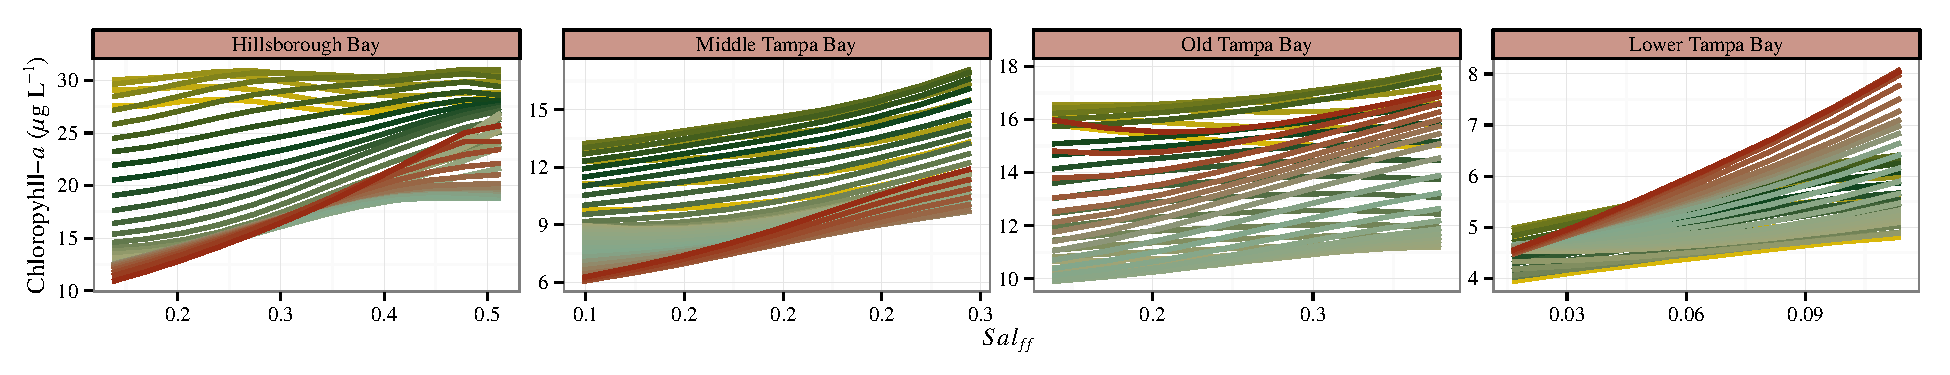
\includegraphics[width=0.9\linewidth]{fig/title_plo.pdf}}

%%%%%%
\begin{frame}[shrink]
\titlepage
\end{frame}

\section{Background}

%%%%%%
\begin{frame}{\textbf{Managing coastal waters}}{\textbf{How do we use data?}}
\emtxt{The good news}: We are getting better at monitoring - standardized, automated, increased coverage, real-time/continuous \\~\\
\emtxt{The bad news}: Our ability to use these data for decision-making has not kept pace with availability! \\~\\


{\centering 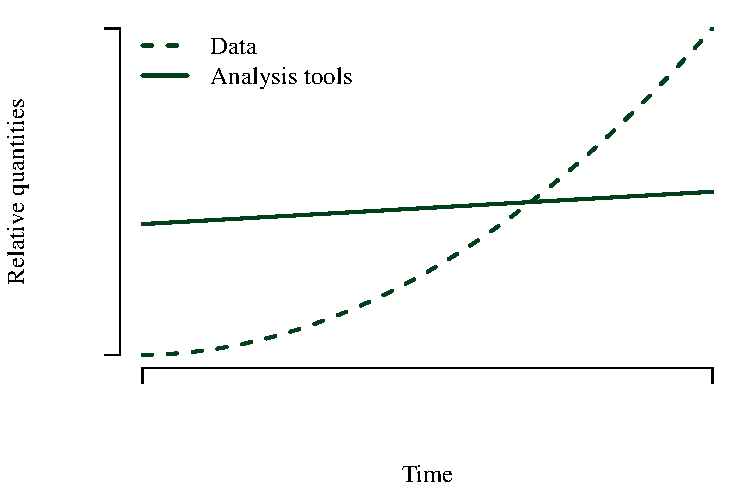
\includegraphics[width=0.55\textwidth]{fig/theo-1} 

}



\end{frame}

%%%%%%
\begin{frame}{\textbf{Managing coastal waters}}{\textbf{How do we use data?}}
\emtxt{Challenge 1:} We have the data but often lack appropriate tools to unambiguously and quantitatively characterize trends \\~\\
\emtxt{Challenge 2:} We must use tools that can leverage the descriptive capabilities of large datasets \\~\\
Our research explores novel techniques to address these challenges:\\~\\
\emtxt{Case 1:} Chlorophyll drivers in Tampa Bay \\~\\
\emtxt{Case 2:} Improving estimates of ecosystem metabolism 
\end{frame}

\section{Case 1: Tampa Bay}

% tampa bay map, w/ inset


%%%%%%
\begin{frame}{\textbf{Case 1: Tampa Bay}}{\textbf{Describing drivers of chlorophyll}}
\begin{columns}
\begin{column}{0.5\textwidth}
\begin{itemize}
\item Four bay segments\\~\\
\item Monthly wq data at 50 stations from 1974 to present \\~\\
\end{itemize}
\vspace{0cm}\hspace*{15pt}\scalebox{0.7}{\hbox{\tiny Data from \cite{TBEP11}}}
\end{column}
\begin{column}{0.5\textwidth}
\centerline{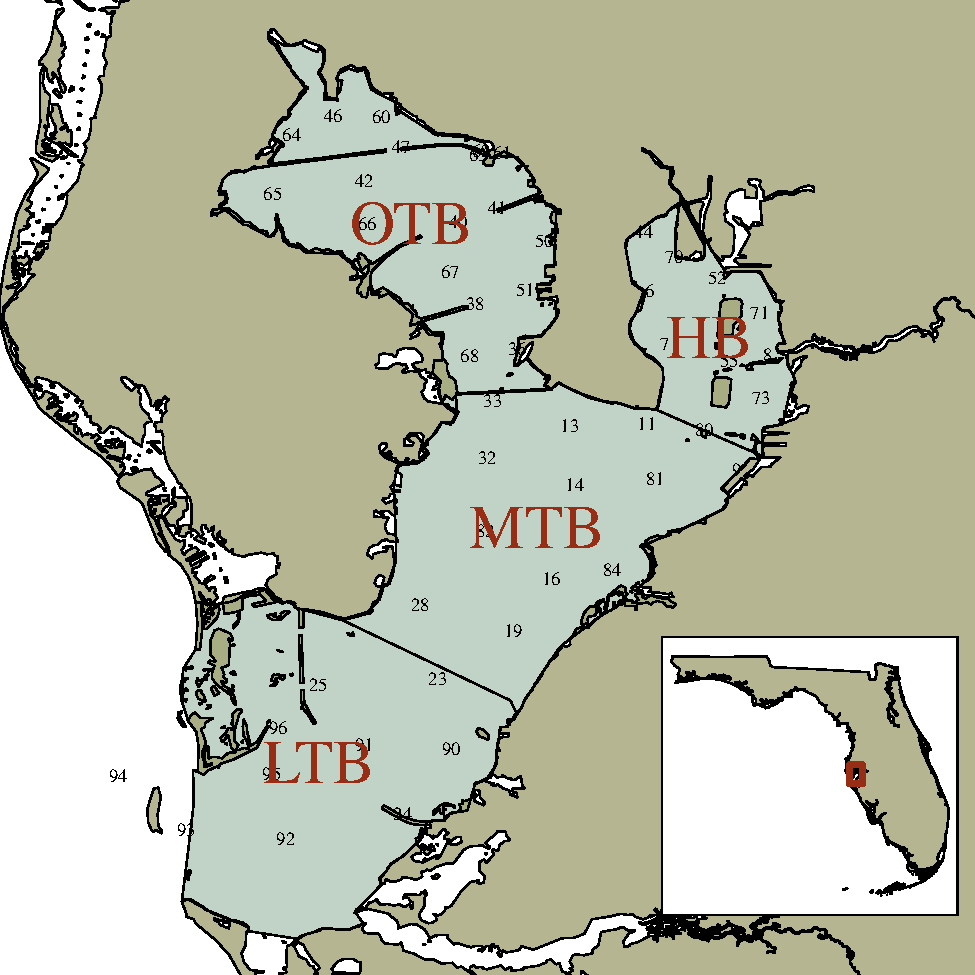
\includegraphics[width = \textwidth]{fig/tb_map.pdf}}
\end{column}
\end{columns}
\end{frame}

%%%%%%
\begin{frame}{\textbf{Case 1: Tampa Bay}}{\textbf{Describing drivers of chlorophyll}}
\begin{figure}[!ht]

{\centering 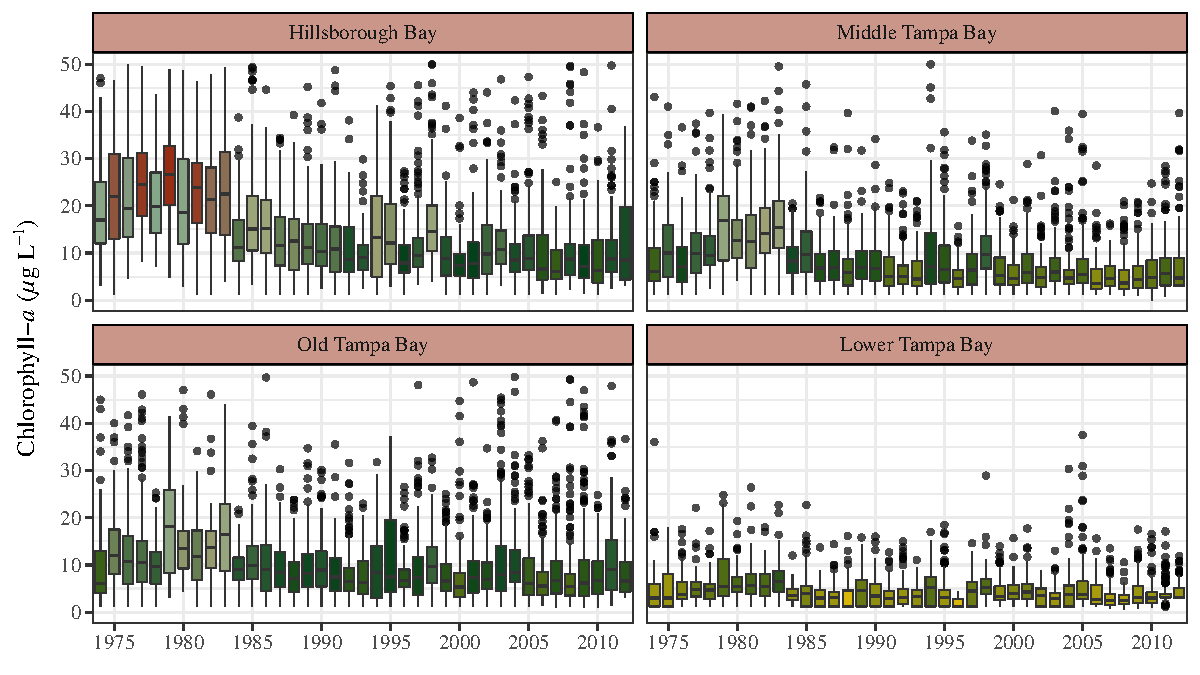
\includegraphics[width=\linewidth]{fig/annual_chl-1} 

}

\caption[Annual trends in chlorophyll for each bay segment]{Annual trends in chlorophyll for each bay segment.}\label{fig:annual_chl}
\end{figure}


\end{frame}

% variation in chl by year, season, and management

%%%%%%
\begin{frame}{\textbf{Case 1: Tampa Bay}}{\textbf{Describing drivers of chlorophyll}}
What affects our interpretation of chlorophyll response to nutrients?
\vspace{-0.1in}
\captionsetup[subfloat]{captionskip=0pt, position=top}
\begin{figure}
\centering
\subfloat[]{
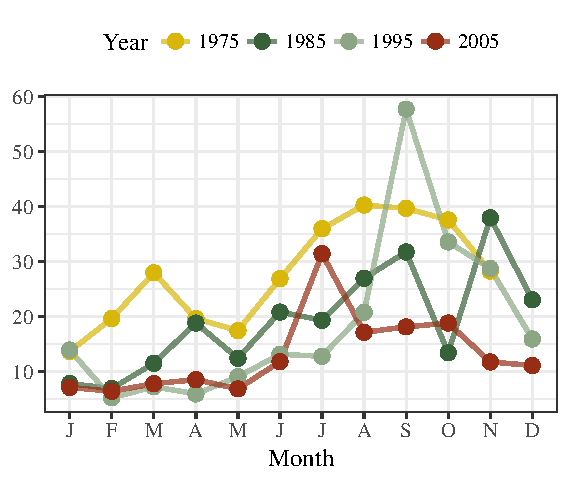
\includegraphics[width=0.46\textwidth,page=1,trim=0.2in 0in 0in 0.35in,clip]{fig/salmoyr.pdf}
\label{fig:salmoyr1}
}
\subfloat[]{
\includegraphics[width=0.46\textwidth,page=2,trim=0.2in 0in 0in 0.35in,clip]{fig/salmoyr.pdf}
\label{fig:salmoyr2}
}

\leavevmode\smash{\makebox[0pt]{\hspace{0em}% HORIZONTAL POSITION           
  \rotatebox[origin=l]{90}{\hspace{3em}% VERTICAL POSITION
    {\color{black} Chlorophyll-\textit{a}}}}}
    \hspace{0pt plus 1filll}\null

\caption{Variation in chlorophyll by {\color{cavalcanti5}\protect\subref{fig:salmoyr1}} time and {\color{cavalcanti5}\protect\subref{fig:salmoyr2}} salinity and management in Hillsborough Bay.  Panel {\color{cavalcanti5}\protect\subref{fig:salmoyr1}} is colored before and after wastewater treatment in 1979.}
\label{fig:salmoyr}
\end{figure}
\captionsetup[subfloat]{position=top}
\end{frame}

%%%%%%
\begin{frame}{\textbf{Case 1: Tampa Bay}}{\textbf{Describing drivers of chlorophyll}}
The \emtxt{weighted regression (WRTDS)} model is being developed by USGS for pollutant modelling in rivers \cite{Hirsch10}\\~\\
Based on the idea that pollution concentration is a function of \emtxt{time}, \emtxt{discharge}, and \emtxt{season}\\~\\
\emtxt{Problem:} We want to see if management has an effect on reducing pollutant load over time, but pollutant load varies with discharge.\\~\\
\emtxt{Solution:} Develop a model that accounts for changes in relationships between drivers of pollution over time.\\~\\
\emtxt{Adaptation:} Can this approach be used to evaluate chlorophyll trends in Tampa Bay?
\end{frame}



%%%%%%
\begin{frame}{\textbf{Case 1: Tampa Bay}}{\textbf{Describing drivers of chlorophyll}}
How does weighted regression work?
\begin{center}
\animategraphics[controls,width=\linewidth]{10}{fig/wtex}{}{} %frame rate is 10 per/sec
\end{center}
\end{frame}



%%%%%%
\begin{frame}{\textbf{Case 1: Tampa Bay}}{\textbf{Describing drivers of chlorophyll}}
Results show temporally consistent trends over time
\begin{figure}
\centerline{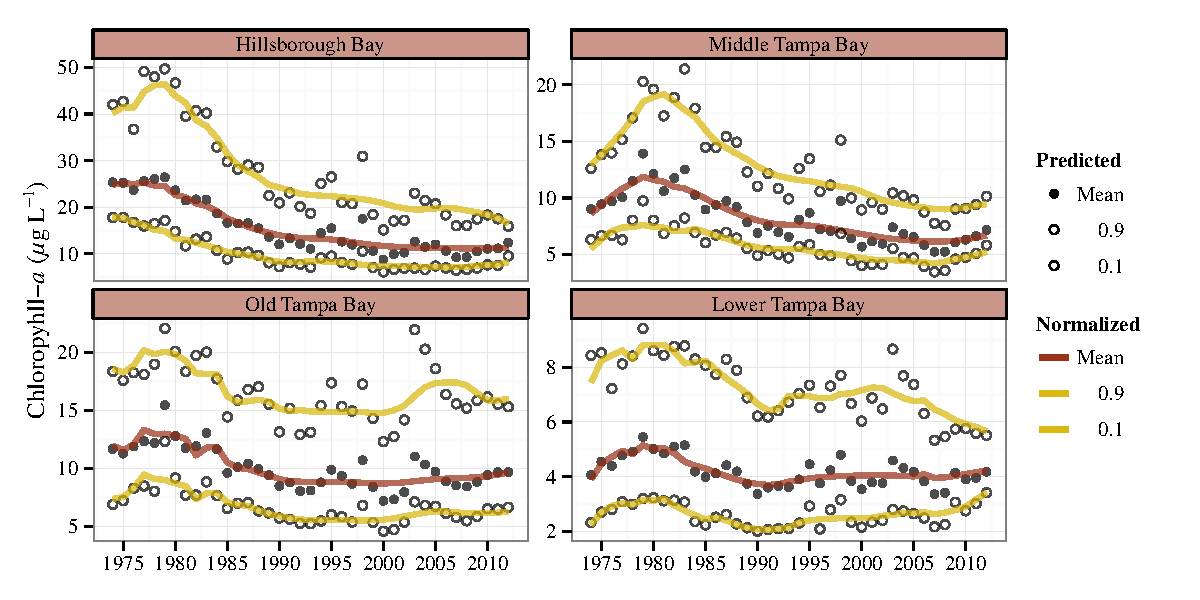
\includegraphics[width = \textwidth]{fig/prdnrm.pdf}}
\caption{Predicted and salinity-normalized annual chlorophyll by segment.}
\end{figure}
\end{frame}

\section{Case 2: Improving metabolism estimates}

%%%%%%
\begin{frame}{\textbf{Case 2: Improving estimates of metabolism}}{\textbf{Application to Gulf Coast estuaries}}
The `Odum' open-water method has been used for decades to estimate rates of ecosystem metabolism \scriptsize \cite{Odum56} \\~\\
\normalsize
\begin{center}
$\frac{\delta DO}{\delta t} = P - R + D$
\end{center}
Metabolic rates provide a measure of productivity in a system - are estuaries sources or sinks of organic matter? \scriptsize \cite{Caffrey14}
\normalsize \\~\\
Applications to estuarine monitoring data have been somewhat successful - why?? 
\end{frame}

%%%%%%
\begin{frame}{\textbf{Case 2: Improving estimates of metabolism}}{\textbf{Application to Gulf Coast estuaries}}
The `Odum' method assumes DO represents biological processes...


{\centering 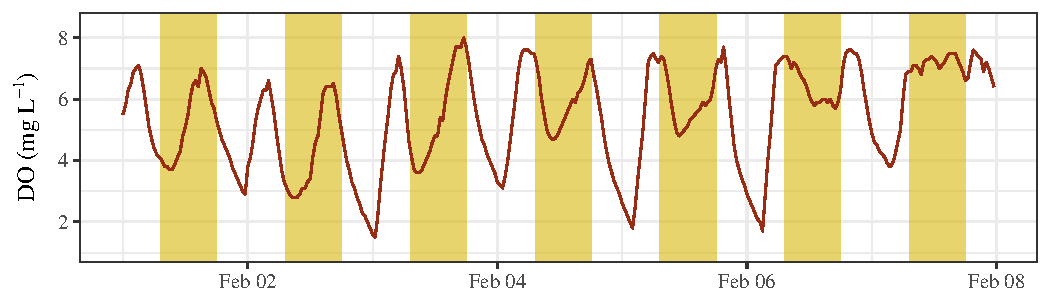
\includegraphics[width=0.95\textwidth]{fig/sapdo-1} 

}





{\centering 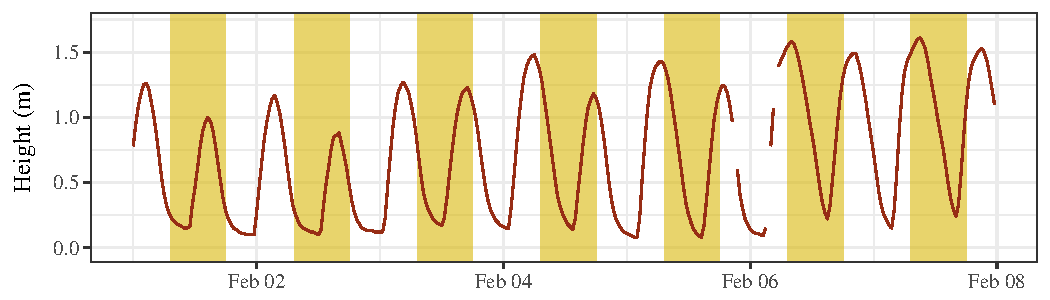
\includegraphics[width=0.95\textwidth]{fig/saptide-1} 

}



\end{frame}

%%%%%%
\begin{frame}{\textbf{Case 2: Improving estimates of metabolism}}{\textbf{Application to Gulf Coast estuaries}}
\emtxt{Challenge:} DO time series may represent variation from physical and biological processes \\~\\
\emtxt{Solution:} The weighted regression approach could be used here...
\vspace{0.15in}
\begin{center}
$\ln\left(Chl\right) = \beta_0 + \beta_1 Sal_{ff} + \beta_2 t $
\end{center}
\vspace{0.05in}
\begin{center}
$DO = \beta_0 + \beta_1 H + \beta_2 t $
\end{center}
\end{frame}

%%%%%%
\begin{frame}{\textbf{Case 2: Improving estimates of metabolism}}{\textbf{Application to Gulf Coast estuaries}}
\centerline{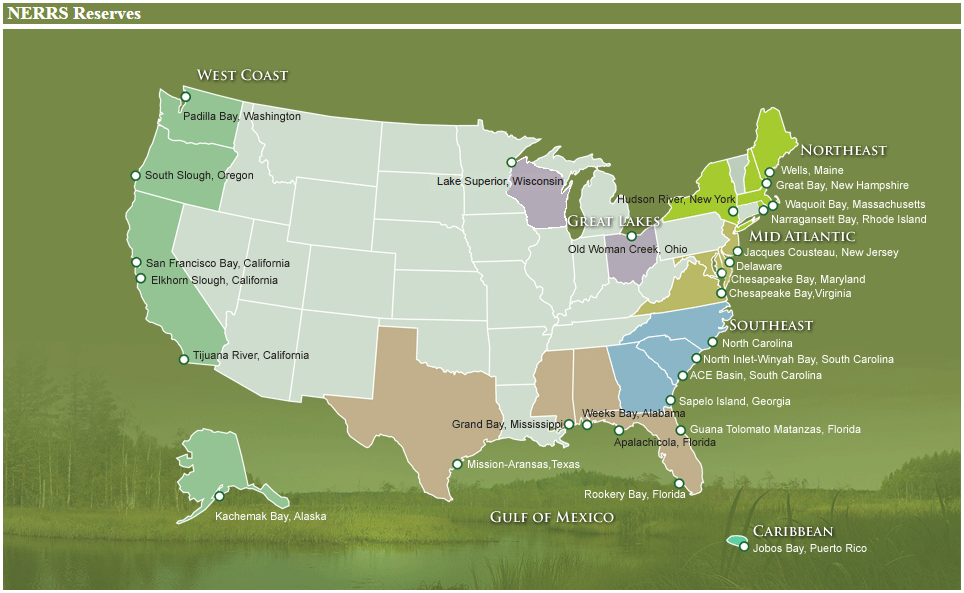
\includegraphics[width = \textwidth]{fig/NERRS_locations.png}}
\end{frame}



%%%%%%
\begin{frame}{\textbf{Case 2: Improving estimates of metabolism}}{\textbf{Application to Gulf Coast estuaries}}
\begin{center}
\animategraphics[controls,width=\linewidth]{50}{fig/detide_ani}{1}{169} %frame rate is 50 per/sec
\end{center}
\end{frame}

\begin{frame}{\textbf{Case 2: Improving estimates of metabolism}}{\textbf{Application to Gulf Coast estuaries}}
\begin{knitrout}
\definecolor{shadecolor}{rgb}{0.969, 0.969, 0.969}\color{fgcolor}

{\centering 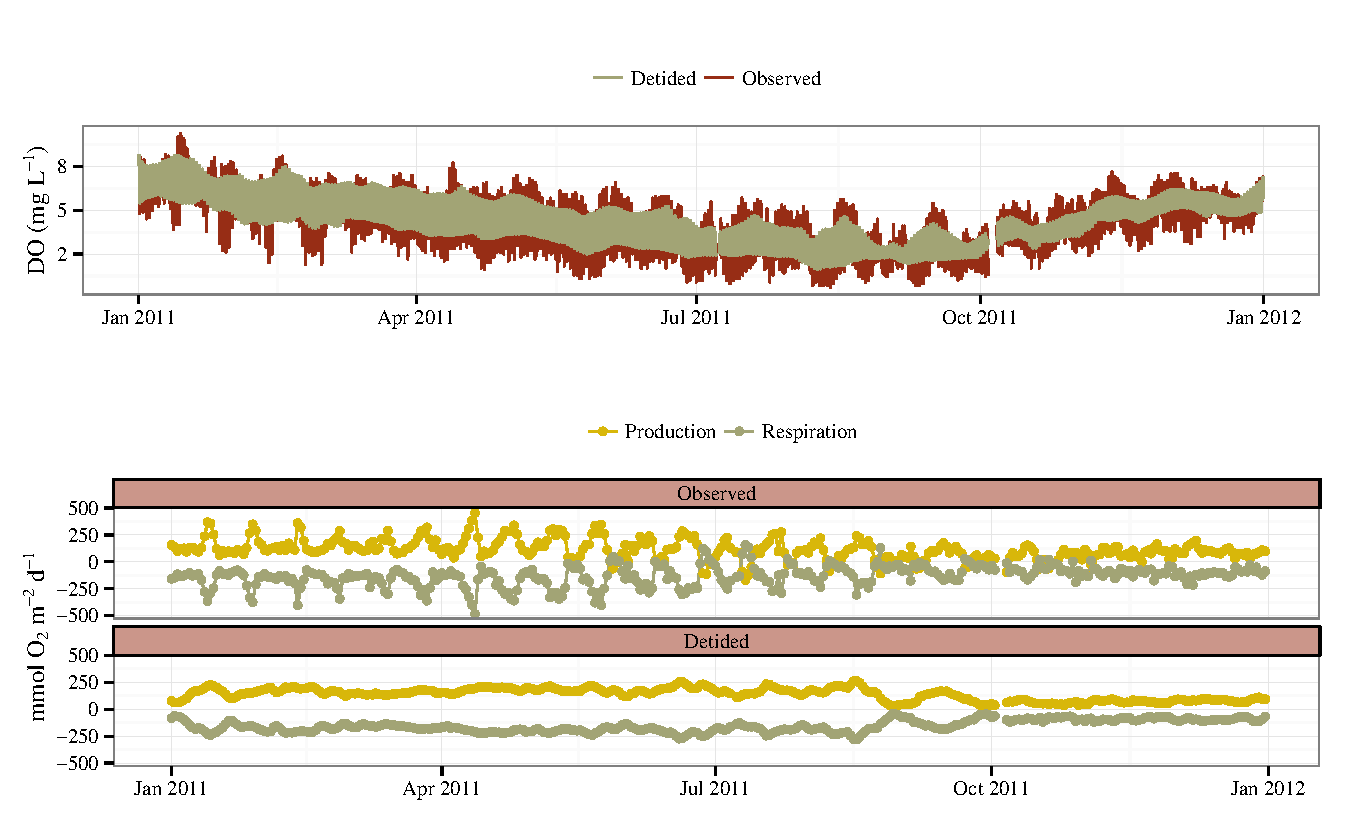
\includegraphics[width=\textwidth]{fig/dtd_met} 

}



\end{knitrout}
\end{frame}

\section{Conclusions}

%%%%%%
\begin{frame}{\textbf{Conclusions}}
The analysis of water quality will continue to require the use of novel techniques, such as weighted regression\\~\\
These needs are motivated by: \\~\\
\begin{itemize}
\item The continued relevance of stressors that influence ecosystem conditions \\~\\
\item Our increasing ability to gather raw, uninterpreted data \\~\\
\end{itemize}
\end{frame}

%%%%%%
\begin{frame}
Acknowledgments:\\~\\
\begin{columns}
\begin{column}{0.6\textwidth}
{\footnotesize
Field staff and data managers at Hillsborough County Environmental Protection Commission, Tampa Bay Estuary Program\\~\\
Research coordinators, technicians, and field staff of the National Estuarine Research Reserve System}\\~\\
\end{column}
\begin{column}{0.3\textwidth}
\vspace{-0.2in}
\begin{center}
{\tiny
Wes Anderson Cavalcanti color theme borrowed and adapted from \href{https://github.com/karthik/wesanderson}{github.com/karthik}\\~\\

\includegraphics[width=0.55\linewidth]{fig/cavalcanti.jpg}\\~\\
\vspace{-0.15in}
\scalebox{0.7}{\hbox{\tiny Image credit:\thinspace{\tiny \href{https://m1.behance.net/}{https://m1.behance.net/}}}}}
\end{center}
\end{column}
\end{columns}
\vfill
Funding sources and contact:\\~\\
\begin{columns}
\begin{column}{0.5\textwidth}
\centerline{
\includegraphics[width=0.4\linewidth]{fig/epa_logo.png}}
\end{column}
\begin{column}{0.5\textwidth}
\scriptsize
\href{mailto:beck.marcus@epa.gov}{beck.marcus@epa.gov} \\~\\
Phone: 8509342480 \\~\\
Github: \href{https://github.com/fawda123/}{github.com/fawda123/} \\~\\
Blog: \href{http://beckmw.wordpress.com/}{beckmw.wordpress.com/}
\end{column}
\end{columns}
\vspace{0.2in}
\end{frame}

%%%%%%
\section{References}
\begin{frame}[allowframebreaks,t]{\textbf{References}}
\footnotesize
\setbeamertemplate{bibliography item}{}
\bibliographystyle{apalike_mine}
\bibliography{ref_diss}
\end{frame}

\end{document}
